%----------------------------------------------------------------------------------------
%	PACKAGES AND OTHER DOCUMENT CONFIGURATIONS
%----------------------------------------------------------------------------------------
\documentclass[fleqn,9 pt]{SelfArx} % Document font size and equations flushed left

% Decrease margins
%\addtolength{\oddsidemargin}{-0.3 in}
%\addtolength{\evensidemargin}{0 in}
%\addtolength{\textwidth}{0.8 in}
%\addtolength{\topmargin}{-0.5 in}
%\addtolength{\textheight}{1 in}

\usepackage[english]{babel} % Specify a different language here - english by default
\usepackage{lipsum} % Required to insert dummy text. To be removed otherwise
\usepackage{listings}
\usepackage{lipsum}  
\usepackage{caption}

%----------------------------------------------------------------------------------------
%	COLUMNS
%----------------------------------------------------------------------------------------
\setlength{\columnsep}{0.55cm} % Distance between the two columns of text
\setlength{\fboxrule}{0.75pt} % Width of the border around the abstract
%----------------------------------------------------------------------------------------
%	COLORS
%----------------------------------------------------------------------------------------
\definecolor{color1}{RGB}{0,0,90} % Color of the article title and sections
\definecolor{color2}{RGB}{0,20,20} % Color of the boxes behind the abstract and headings

%----------------------------------------------------------------------------------------
%	HYPERLINKS
%----------------------------------------------------------------------------------------
\usepackage{hyperref} % Required for hyperlinks
\hypersetup{hidelinks,colorlinks,breaklinks=true,urlcolor=color2,citecolor=color1,linkcolor=color1,bookmarksopen=false,pdftitle={Title},pdfauthor={Author}}

%----------------------------------------------------------------------------------------
%	ARTICLE INFORMATION
%----------------------------------------------------------------------------------------
\JournalInfo{Project 2 - CS-433 - Road Classification with 2D Convolutional Neural Networks} % Journal information
\Archive{\today} % Additional notes (e.g. copyright, DOI, review/research article)

%%%%% dumb test
\usepackage[english]{babel}
\usepackage{blindtext}

\PaperTitle{Road Classification with 2D Conv. Neural Networks} % Article title

\Authors{Bruno Magalhaes\textsuperscript{1}, Riccardo Silini\textsuperscript{2} \hspace{7.7cm} team: OhWell} % Authors
\affiliation{\textbf{Email (SCIPER):} \hspace{0.2cm} \textsuperscript{1} bruno.magalhaes@epfl.ch (212079) \hspace{0.2cm} \textsuperscript{2} riccardo.silini@epfl.ch (214398) \hspace{0.2cm}}

\Keywords{}
%Keyword1 --- Keyword2 --- Keyword3

\newcommand{\keywordname}{Keywords} % Defines the keywords heading name

%to allow overlapping
\usepackage[percent]{overpic}
\usepackage[]{algorithmic,algorithm2e}

%to allow \figures right below text 
\usepackage{float}

%---------- ABSTRACT

\Abstract{ Road classification from orthogonal aerial photographies allows for automatic reconstruction of maps, guidance of autonomous vehicles, among others. Manual classification is infeasible due to the large amount of information and work involved. Automatic classification can be pursued with Machine Learning techniques. With that in mind, we present an algorithm for the automatic labelling of roads from sets of pictures using a 2D convolutional neural network. For added accuracy, we improve the provided sample code with data augmentation and dropout techniques and a 2-step neural network processing that learns from predictions of road labels.}

\begin{document}
\begin{sloppypar} %allows line breaks in \texttt{---} section

\flushbottom % Makes all text pages the same height
\maketitle % Print the title and abstract box
\tableofcontents % Print the contents section
%\thispagestyle{empty} % Removes page numbering from the first page

\section{Introduction}

Road segmentation, classification and detection has received large interest in the last years. Its applications range from autonomous vehicles, tracking devices, and other mechanisms that automate the navigation of a wide scope of guidance devices. The large amount of data to be processed and the complexity of a proper interpretation is a bottleneck due to difficulty in achieving an accurate interpretation of a wide scope of information. For simplicity, most common application utilise freely available collections of aerial photographies. Manual interpretation of such images is infeasible, therefore automated techniques such as regression, edge detection, variance of features and computer vision are used.

In this document, we present an automatic method for the classification of roads from given satellite photography images, based on Machine Learning techniques. The classifier is implemented on a 2D convolutional neural network, built with the TensorFlow API. The architecture of the convolutional network of weights is based on several layers of convolution followed by two layers of fully connected nodes. The input is described by a square patch of RGB pixels, where patches are collected from the set of aforementioned images. The patches are described by the segments to be labelled and an additional margin of surrounding pixels that describe the neighborhood information. The output is the probability of a given input being classified as road and non-road.

The parameters of the execution and the Stochastic Gradient Descent algorithm are detailed in the following sub-section. Added accuracy was introduced by several features tuning of parameters, patches neighborhood information, several layers of convolution, randomizing and balancing of input data per label, dropout and two networks that learn (1) from the input patch and (2) from the prediction of the previous patch labelling, respectively, with the latter serving the purpose of providing noise reduction.

For higher precision, we increased the input size with two data augmentation techniques, generating new image patches from pre-existing rotated patches, and from filtering patches from interleaved intervals of existing patches, as detailed in Section \ref{sec-data-augmentation}.

We evaluated our results on a Macbook Air 13.3" 2015 and collected the feedback from the Kaggle system page, as presented in the results section (\ref{sec-results}). Section \ref{sec-conclusion} draws final conclusions.

\begin{figure*}
\centering
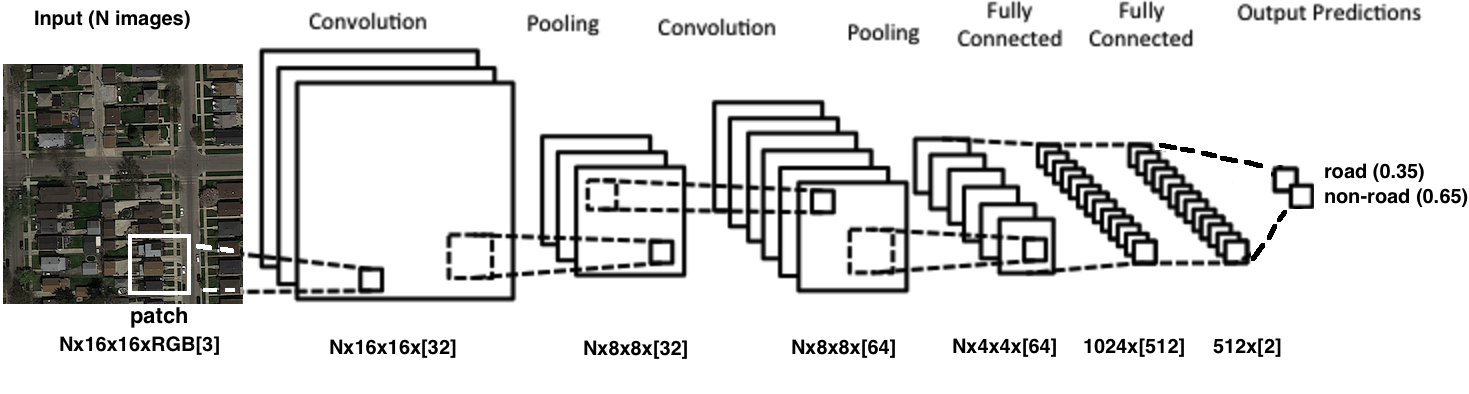
\includegraphics[width=1\textwidth]{figures/conv_2d_network.png}
\caption{A general overview of the deep network architecture, with default parameters. Dimensionalities, padding types, depths and number of convolution+pooling layers are user-customisable.}
\label{fig-conv-2d-architecture}
\end{figure*}

\paragraph{Execution Parameters}
\label{sec-execution-parameters}

The gradient descent algorithm parameters are the following: \texttt{LEARNING\_RATE} specifies the step size on the gradient descent update, with a decay given by \texttt{DECAY\_RATE}; the iterations count is defined in \texttt{NUM\_EPOCHS}; the value set by the variable \texttt{BATCH\_SIZE} specifies how many input elements are to be used on the weights update, in practice allowing one to run Stochastic Gradient Descent by inputting a single element, a batch of elements, or all input data; \texttt{INPUT\_SIZE} sets the number of images used for training.

For labelling, \texttt{FOREGROUND\_THRESHOULD} defines the threshold of the mean gradient on a given patch to be considered as non-road;

Multi-core processing is possible by setting \texttt{NUM\_THREADS} to the respective value of maximum concurrent threads in the processor's architecture. \texttt{SEED} allows one to reproduce results by setting the random seed to the given value. The model training is stored automatically at every set of \texttt{RECORDING\_STEPS} steps. A model can be restored by setting the flag \texttt{RESTORE\_MODEL} to \texttt{True}.

\section{Architecture}

Our network is composed by a set of convolution layers (for extracting of convoluted features) and pooling layers (for the extraction of most meaningful weights from convolutional layer outputs), followed by two layers of fully connected layers (the universal function approximators). The input is a set of images to which patches are extracted. Those patches are then input individually or in batches to the network. The output contains the probability of the road or non-road classification. A sample of a possible network architecture with 2 convoluted layers and default parameters is displayed in figure \ref{fig-conv-2d-architecture}.

\paragraph{Multi-Layer convolutional network}

We allow the sub-network of convolution layers to increase or decrease, according to the user-defined parameters \texttt{CONV\_LAYERS}. This allowed us to play with the quality of model fitting for different sets of parameters. In practice, our network is an array of convolution and pooling layers, where the output of one layer is the input of the following one. The quality of fitting is defined by a set of user-provided filter sizes, depths and strides per layer, and number convolution of layers. Such information is represented by the following variables:
\begin{itemize}
\item \texttt{CONV\_LAYERS}: number of convolutional layers, and size of the following parameter arrays;
\item \texttt{CONV\_FILTER\_SIZES = [5,5,5,5]} : For each layer, the count of horizontal and vertical pixels of filter;
\item \texttt{CONV\_FILTER\_DEPTHS = [32, 64, 128, 256]}: depth of the weights for the aforementioned layers;
\item \texttt{POOL\_FILTER\_STRIDES = [2, 2, 2, 2]}: horizontal and vertical stride for the max-pooling on each layer;
\item \texttt{FC1\_WEIGHTS\_DEPTH = 512}: depth of the first fully connected layer, connected to conv. layer of id \texttt{CONV\_LAYERS-1}. The second layer performs binary probability classification therefore has depth \texttt{NUM\_LABELS} (road; non-road);
\end{itemize}
  A multi-layer network allowed us to work with a finer detail on the images, specifically to look into patches of a smaller \text{IMG\_PATCH\_SIZE}. This allowed us to play use the noisy version output from a small grain classification as an input to the second network, as detailed in the following paragraph.

\begin{figure}[H]
\centering
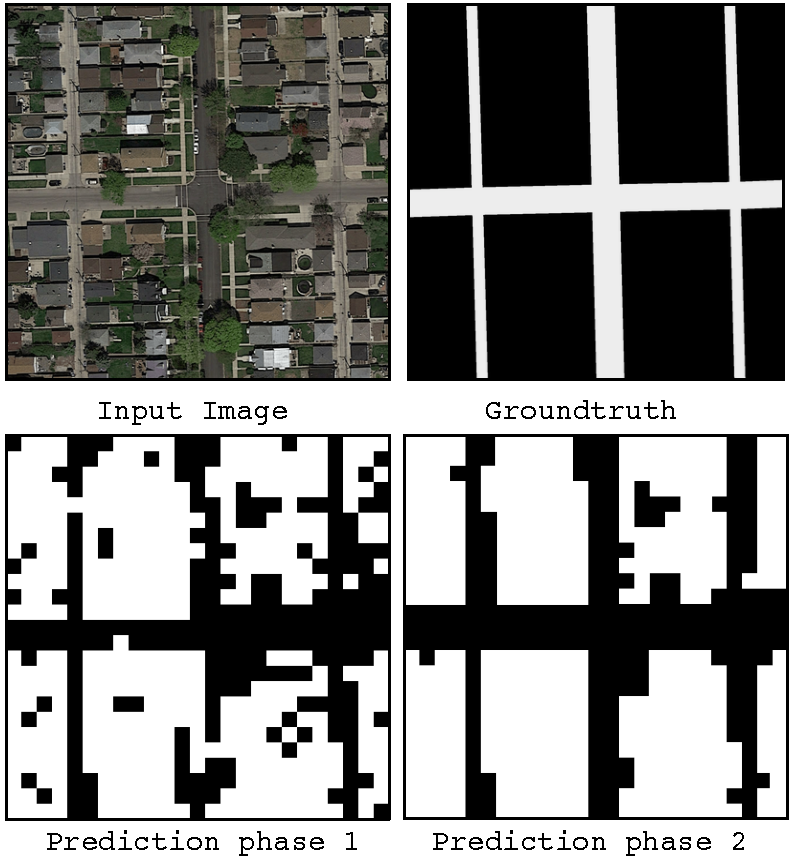
\includegraphics[width=0.3\textwidth]{figures/two_phases_conv2d.pdf}
\caption{An example of the application of the two-phase propagation process: for a given input (top-left), the predicted segmentation at output of the neural network (bottom-left) is then re-input to a second neural network trained from groundtruth images (top-right), outputting the final classification (bottom-right).}
\end{figure}

\paragraph{Two-step classification} 

To reduce noise and allow classification at a finer scale, we added a second neural network to the processing. The workflow is the following: the initial layer is trained with pairs of [images,groundtruth] and outputs the segmented classification. The second network is trained with pairs [classification,groundtruth] and receives the first network's classification as input, outputting the final classification. The second step of this operation is presented as \texttt{Phase 2} in the source code. In practice, it increases accuracy of prediction by cleaning noise (\textit{lonely} labels) from input. Among all the filters provided by this process, the most relevant properties are (1) filter out unconnected roads, (2) filter our roofs with similar patterns as roads, (3) labelling of road to cars and trees on the road. An example of an application of the two-step classification is displayed in the following picture.


\paragraph{Analysis of neighborhood information} Classification of a patch based on the surrounding pixels had been shown to increase the accuracy rate of the network when applied previously to Logistic Regression methods (LR). Nevertheless, LR did not allow for enough depth of the network to universally approximate the problem --- in practice equivalent to a fully-connected \textbf{single-layer} neural network. We moved this functionality to our network by introducing \texttt{VALID} padding to the first convolutional layer of nodes and using as a patch to be classified and its neighborhood. To allow classification of side or corner patches we introduce a margin of \textit{zeroed} RGB pixels around the patch. This functionality can be activated wit the flag \texttt{NEIGHBORHOOD\_ANALYSIS} set to \texttt{True} and definining the \texttt{NEIGHBOR\_PIXELS} to the margin of neighborhood pixels to be added and analysed from each patch. In practice, input patches are of size \texttt{IMG\_PATCH\_SIZE+NEIGHBOR\_PIXELS*2} squared, providing better classification yet adding extra computational time to the training process.

\begin{figure}[H]
\centering
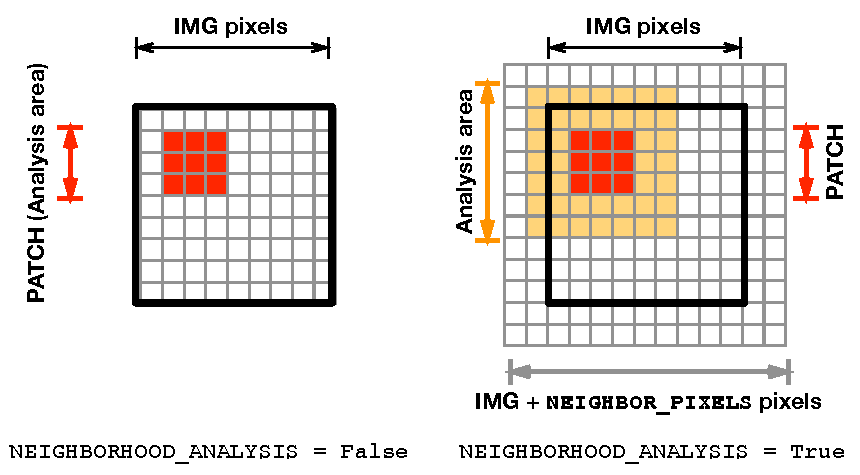
\includegraphics[width=0.47\textwidth]{figures/NEIGHBORHOOD_ANALYSIS.pdf}
\caption{Example of the neighborhood analysis feature. Standard classification (left) inputs patches of images and classifies the same area (red). With neighborhood analysis (right), we input the patch of size \texttt{IMG\_PATCH\_SIZE} and all surrounding \texttt{NEIGHBOR\_PIXELS} pixels (orange), with the learning based on the labels of the patch only (red).}
\end{figure}

\paragraph{Balanced and Randomized input sequence}

The order in which we present the observations (input vectors) comprising the training set to the network affects the final computation of weights. We implemented a randomized arrangement of the observations according to the response variable that has been shows to be present a better tuned network when compared with ordered arrangements (the standard implementation). Our input is then a randomized set of classification with balanced number of inputs for each label. This feature is enabled by defining \texttt{RANDOMIZE\_INPUT\_PATCHES = True}.

\paragraph{Dropout}

Dropout is a regularization technique for reducing the overfitting of neural networks. It performs model averaging of neural networks efficiently and prevents complex co-adaptations on training data (Srivastava et at. 2014 \cite{srivastava2014dropout}). We enabled dropout in our models by specifying the percentage of dropout on the variable \texttt{DROPOUT\_RATE} as exemplified in the next figure:

\begin{figure}[H]
\centering
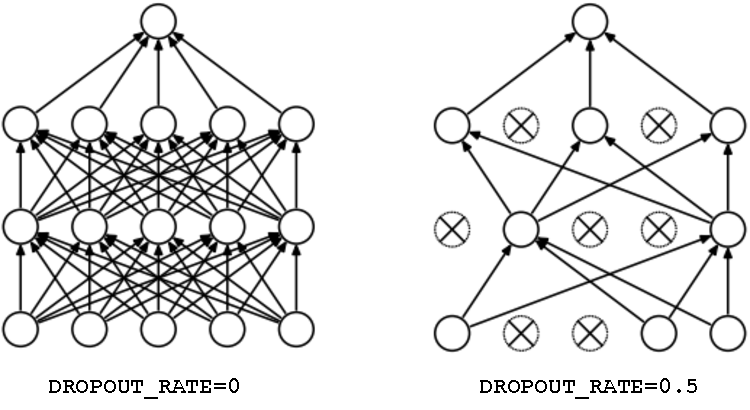
\includegraphics[width=0.44\textwidth]{figures/DROPOUT_RATE.pdf}
\caption{Example of the dropout feature. Standard weights tunning (left) methods apply an update of all weights. Dropout-based networks (right) discards the updates of certain weights with the rationale of reducing overfitting. In the example, a dropout rate of \texttt{0.5} disables half of the nodes on the network.}
\end{figure}


\section{Data Augmentation}
\label{sec-data-augmentation}

To allow for a larger input set, and better tuning or weights, we introduced two data augmentation techniques, presented next.

\paragraph{1. Rotation of input images with non-orthogonal roads} We increased the number of input images from $100$ to $148$ by rotating $90 \deg$, $180 \deg$ and $270 \deg$ the (16) training images that are not composed only of non-horizontal and non-vertical roads. This feature is activated by the flag \texttt{DATA\_AUGMENTATION}.

\paragraph{2. Patches from concatenation points} We increase by almost two-fold the number of patches per training image by performing extraction of all patches of size \texttt{IMG\_PATCH\_SIZE} that are placed at every \texttt{IMG\_PATCH\_SIZE/2} interval. This feature is activated by the flag \texttt{ADD\_INTERCALATED\_PATCHES}. In practice, it extracts patches with the corners at the mid-point positions of previously extracted patches, as displayed below:

\begin{figure}[H]
\centering
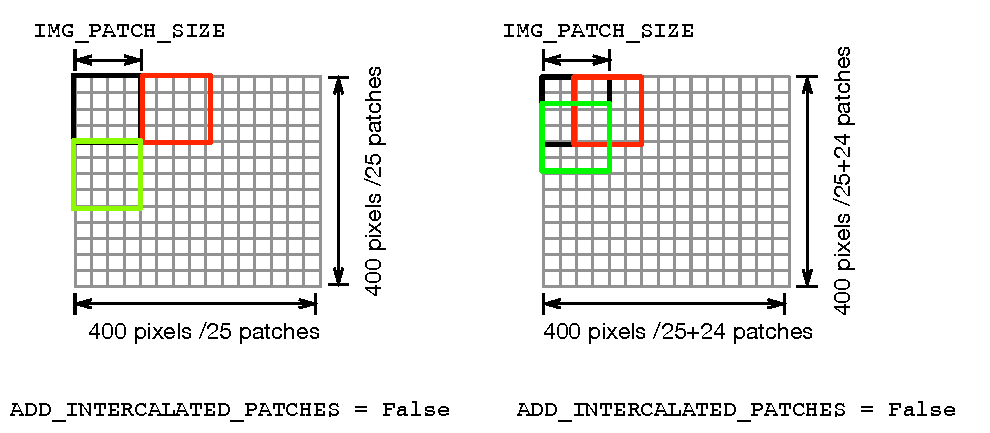
\includegraphics[width=0.47\textwidth]{figures/ADD_INTERCALATED_PATCHES.pdf}
\caption{The collection of patches by stepping \texttt{IMG\_PATCH\_SIZE} (default, left) compared with \texttt{IMG\_PATCH\_SIZE/2} (\texttt{ADD\_INTERCALATED\_PATCHES} activated, right). When traversing image, next collected patch on the horizontal (vertical) direction is displayed as red (green).}
\end{figure}

\section{Analysis of Performance and Conclusion}
\label{sec-conclusion}

Fine tuning of convolutional neural networks for the classification of roads is a highly sophisticated process. In this document, we presented the main issues such as high variability and noise that are present in such problems, and presented some resolutions. Moreover, we added some features that were presented in similar resolutions, particularly the neighborhood information analysis applied in Logistic Regression. We explored a feedback mechanism that learns from wrong vs correct predictions and allows road classification to be further improved by cleaning unrealistic scenarios such as unconnected patches of roads, and roofs with similar properties as roads. We studied different architectures and isolated the parameters that allow for possible configurations of such networks. The high level of free variables and data required (particularly when adding neighborhood) requires high processing power for a good search of suitable parameters. When tuned individually, such parameters deliver a good improvement when enabled. Nevertheless, the combination of parameters did not yield the perfectly linear increase of accuracy, as expected. The best fitting of parameters based on individual metrics of parameters is not enough, possibly requiring a grid search or other approaches for better results. Moreover, our training was performed on a laptop during 5h and 10 epochs, which in our opinion is not sufficient, thus requiring larger step sizes for a faster yet \textit{sloppy} solution. We scored circa 82\% on the Kaggle system. Nevertheless, is our opinion that the parameters presented require further tuning and our scored could have been improved with less time and hardware limitations.

%references
\bibliographystyle{unsrt}
\bibliography{report}

\end{sloppypar}
\end{document}